\chapter*{Choices in Technologies}
\label{ch:techchoices}
In this chapter, we outline the technologies we choose, and the reasoning for choosing them.

\section{Backend}
\label{sec:techbackend}
It is implemented using the Play Framework\cite{playframework} and the Scala\cite{scalalang} programming language.
TODO explain why.

\section{Frontend}
\label{sec:techfrontend}

Given that the frontend must support the three desktop operating systems Microsoft Windows, GNU/Linux as well as Apple MacOS,
the technological choices available to us are limited.
On the desktop, we could use the \gls{JVM} platform and the JavaFX \gls{GUI} library, whereas on the phones
we could use Flutter\cite{flutterframework}.
However, developing three applications on five platforms using two new-to-us frameworks and programming languages
would take a lot more time and resources than what is available to us in the scope of this thesis.

In order to reduce complexity we decide to implement the frontend as a web application, capable of running
in any modern web browser regardless of platform, be it mobile or desktop.
We're not happy about this, as we would much rather use mature, strongly-typed and well-designed languages and frameworks,
but we're forced to make this compromise in order to meet our objectives in the time available.

\subsection{Client-Side File Hashing in the Web Browser}
\label{subsec:browserhashing}
This choice presents us with a challenge: hashing the files to be signed client-side.
If we had implemented "proper" client applications this would've been easy, but in a web browser and its
JavaScript language not so much: they weren't designed with file I/O and CPU-intensive cryptographic functions in mind.
The easiest solution would be to upload the files to be signed to the server and hash them there,
but this would be a clear violation of the least-information principle (the server doesn't need the file, only the hash)
and a breach of user privacy.
Another solution would be to ask the user to enter the file hashes instead of selecting files,
but this would be very user-unfriendly and probably downright impossible for many people.

It is clear we must find a way to hash files in the web browser itself.
In order to achieve this we have found the following options:

\begin{enumerate}
    \item Using the browser-implemented \texttt{SubtleCrypto}\cite{subtlecrypto} \gls{API}
    \item Using the \texttt{CryptoJS}\cite{cryptojs} JavaScript implementation
    \item Using a \gls{WASM}-based implementation
\end{enumerate}

Each of these options comes with a number of advantages and disadvantages, as shown in detail in the following sections.

\subsubsection{Using SubtleCrypto}
\label{subsubsec:subtlecrypto}
The \texttt{SubtleCrypto} class offers the \texttt{digest(algorithm, data)} method, which can be used to
calculate the \gls{SHA-256} checksum of the given data.
The advantage of using this implementation is that it is available in all modern browsers\footnote{Where modern browsers means Mozilla Firefox, Google Chrome/Chromium, and Microsoft Edge},
and since it's executed with native code instead of JavaScript it's quite fast.
There's a major drawback though: hashing a large amount of data progressively is not supported, the data has to be
passed to the function en bloc, as seen in listing~\ref{lst:subtlecrypto}.

\begin{lstlisting}[caption={Using SubtleCrypto for calculating SHA-256 checksums}, captionpos=b, language=JavaScript, label={lst:subtlecrypto}]
crypto.subtle.digest("SHA-256", data).then(hash => {
    console.log(
        // convert ArrayBuffer to hex string
        Array.from(new Uint8Array(hash)).map(
            b => b.toString(16).padStart(2, '0')
        ).join('')
    );
});
\end{lstlisting}
Our testing showed that selecting files larger than 200MB crashes Firefox tabs when trying to read their contents
into memory before we could pass it to the \texttt{digest} function.
If we assume the users will only ever select small files this should not pose a problem, but unfortunately it's not safe to assume this.

\subsubsection{Using CryptoJS}
\label{subsubsec:cryptojs}
\texttt{CryptoJS} does not have the limitation of \texttt{SubtleCrypto} and supports progressive hashing,
as seen in listing~\ref{lst:cryptojsprogressive}.
Progressive hashing is the ability to pass to the hash function the data piece by piece in order to avoid holding all
of it in memory at once.

\begin{lstlisting}[caption={Progressive SHA-256 hashing using CryptoJS},captionpos=b,language=JavaScript,label={lst:cryptojsprogressive}]
const sha256 = CryptoJS.algo.SHA256.create();

sha256.update("Message Part 1");
sha256.update("Message Part 2");
sha256.update("Message Part 3");

const hash = sha256.finalize();
\end{lstlisting}

The advantage of using \texttt{CryptoJS} over \texttt{SubtleCrypto} is as mentioned the ability to hash piece-wise.
The disadvantage is that we need to load a third-party JavaScript library, using built-in functionality would be preferable.
And since JavaScript is an interpreted language, using it to calculate the checksums would presumably result in slower speeds.


\subsubsection{Using a WASM-based implementation}
\label{subsubsec:wasmhashing}
\gls{WASM} provides a low-level virtual machine running machine-independent binary code, comparable to the \gls{JVM} or the \gls{CLR}, albeit much simpler and much less sophisticated.
By using this virtual machine we should be able to, in theory, run code at near-native speed written in a statically-typed, compiled language such as Rust, C++ or Go.
We expect significant speed gains over a JavaScript-based implementation due to the fact that JavaScript is interpreted and untyped\footnote{It's not really untyped, but its type system is so \textit{unique} it might as well not have types.}.
While developing the \gls{WASM}-based hashing program, we encountered some interesting challenges, as described in the following paragraphs.

\paragraph{CORS Policy} While JavaScript can be executed simply by pointing the browser at a local \gls{HTML} file, the same doesn't work for \gls{WASM}.
The browser's security policy forbids it due to its \gls{CORS} rule~\cite{cors}.
We solved this by starting the \gls{HTTP} server built in to Go's standard library and having the browser load the \gls{WASM} binary through \gls{HTTP}.
The code is in appendix TODO put code in appendix and link here.

\paragraph{JavaScript/WASM Compatibility} The Golang project conveniently provides a file containing the necessary boilerplate code to load, start and interact with \gls{WASM} programmes called \texttt{wasm\_exec.js}.
But there's a catch: for each version of Go, the version of the accompanying \texttt{wasm\_exec.js} file used must match precisely.
If it doesn't, the code will crash with a segmentation fault.
It took us quite some time to figure out why the code we'd written only a few days prior would segfault now with no changes made to it.

\paragraph{Passing data} Functions written in Go intended to be used from the JavaScript side of things need to have a very specific signature:

\begin{lstlisting}[caption={Golang WASM function signature}, captionpos=b, language=Go, label={lst:funcsignaturewasm}]
    blubber
\end{lstlisting}


\subsection{Performance Comparison}
\label{subsec:perfcomphashing}
No one likes waiting for slow software to do its work, and neither do we.
Thus we decided to compare the performance of the aforementioned options in a simple test:
we measure the time it takes for the browser to calculate the checksum of 1GB of random data using the three aforementioned methods.
The code used for each example is in appendix TODO add test code and link here.
The tests were run on Debian 10 using Firefox 69 on an Intel i7-8550U.
The results can be seen in figure~\ref{fig:hashingperformance}.
It is obvious we were mistaken: the WASM implementation is significantly slower than the JavaScript implementation.
What really surprised us though was that the browser itself appears to be slower than CryptoJS too.

\begin{figure}
    \begin{center}
        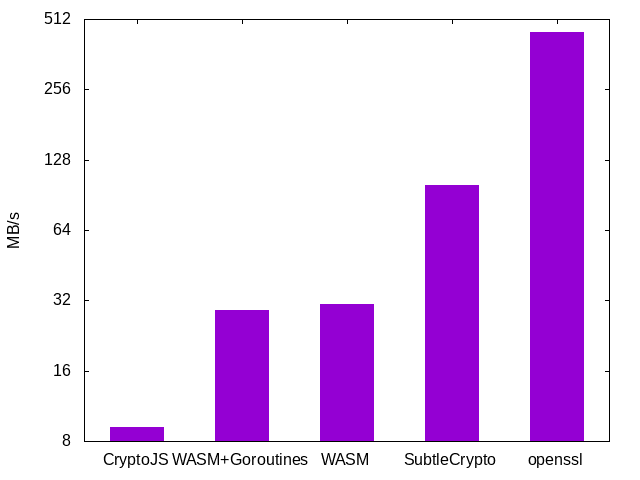
\includegraphics[width=0.7\linewidth]{images/hashingperformance.png}
        \caption{Time in seconds for hashing 1GB of random data}
        \label{fig:hashingperformance}
    \end{center}
\end{figure}


\subsection{Deciding On The In-Browser Hashing Implementation}
\label{subsec:deciding-on-the-in-browser-hashing-implementation}
It is clear from figure~\ref{fig:hashingperformance} that CryptoJS is significantly faster than the other options we tried.
Given that it supports piece-wise hashing as well,
something we need for larger files (as discussed in section~\ref{subsec:browserhashing}), the choice is clear.
We will use CryptoJS to hash the input files in the browser.













